%!TEX root = ../document.tex

\section{Oppgaver 13.11.2013}
\begin{figure}[H]
\centering
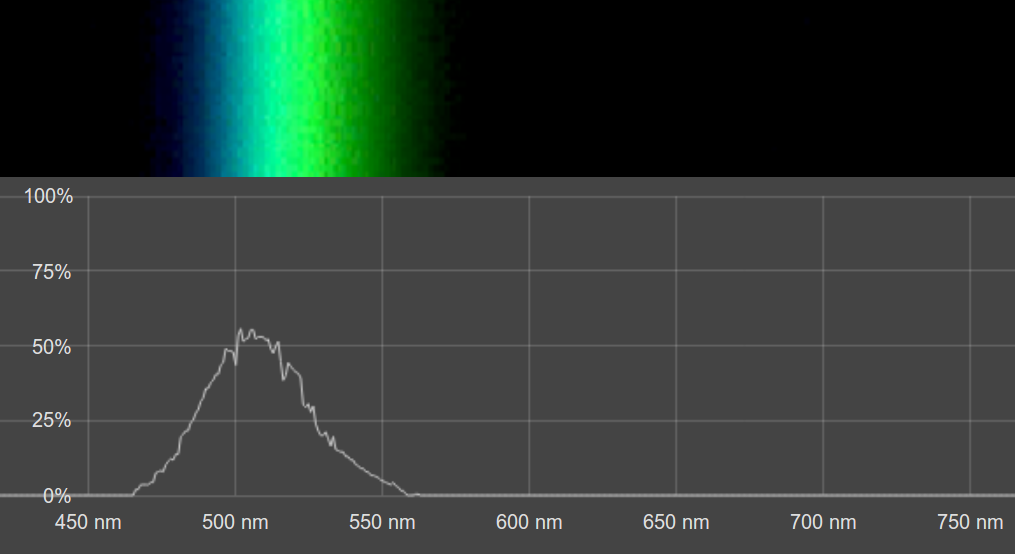
\includegraphics[width=\textwidth]{img/photosynthesis/spectrometer.png}
\end{figure}
\begin{enumerate}
	\item De siste ukene har dere gjennomført to eksperiment. Beskriv eksperimentene.
	\begin{enumerate}
		\item Hva forventet dere kom til å skje?
		\item Hva skjedde?
		\item Dersom det var noen forskjell i resultatene, hva kan årsaken ha vært?
	\end{enumerate}

	\item Se først på videoen fra tirsdag, 29.oktober, så videoen fra 4. november. 
	\begin{enumerate}
		\item Ser dere noen forskjell i hvordan planten beveger seg. 
		\item Dersom ja, hvorfor?
	\end{enumerate}

	\item Se på grafen over jordfuktighet under hele perioden. Plante 1 ble sådd 25.10, og plante 2 ble sådd 1.11. 
	\begin{enumerate}
		\item Er det noen forskjell i absorbasjonsraten?
		\item Hva kan årsaker til dette være?
		\item Grafen flater ut mot slutten av perioden. Hva kan årsaker til dette være?
		\item Er det mulig å bruke jordfuktighet som mål for raten av fotosyntese?
	\end{enumerate}

	\item Se på vekstraten til de to plantene. 
	\begin{enumerate}
		\item Hvilken plante vokser raskest?
		\item Hvorfor?
		\item Er det noen ulikheter i bladenes utseende?
	\end{enumerate}

	\item Se på den siste videoen og sammenlign med video fra mandag 4.nov.
	\begin{enumerate}
		\item Hva har skjedd med vekstraten?
		\item Hvorfor?
	\end{enumerate}
\end{enumerate}

\begin{figure}[H]
\centering
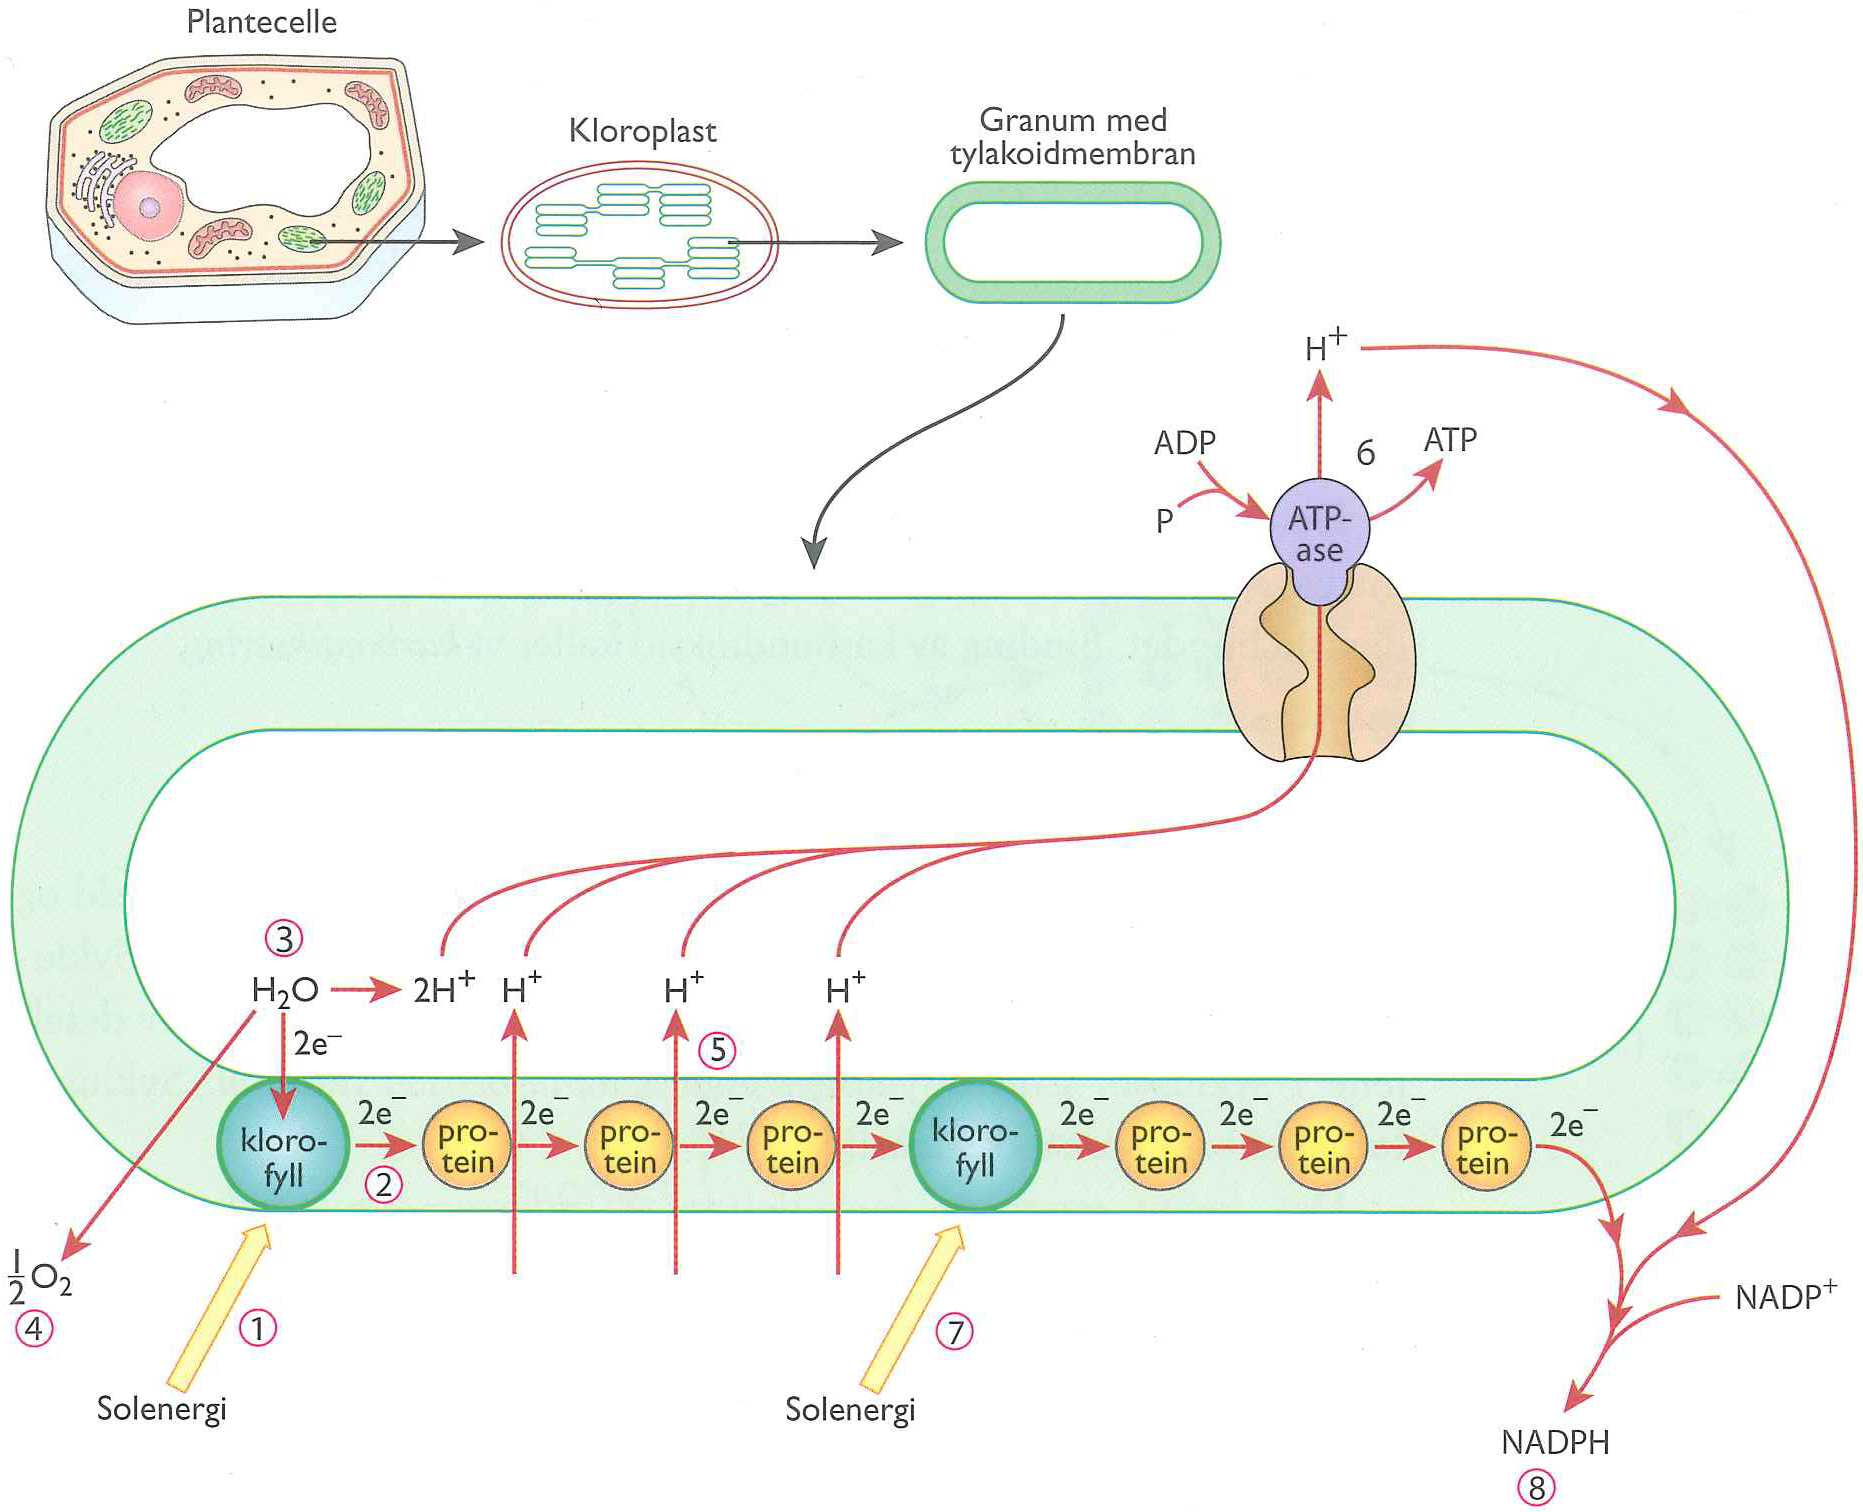
\includegraphics[width=\textwidth]{img/photosynthesis/light_dependent.png}
\end{figure}